\documentclass[10pt]{article}
\usepackage[polish]{babel}
\usepackage[utf8]{inputenc}
\usepackage[T1]{fontenc}
\usepackage{amsmath}
\usepackage{amsfonts}
\usepackage{amssymb}
\usepackage[version=4]{mhchem}
\usepackage{stmaryrd}
\usepackage{graphicx}
\usepackage[export]{adjustbox}
\graphicspath{ {./images/} }

\title{KLASY PO SZKOLE PODSTAWOWEJ }

\author{}
\date{}


\begin{document}
\maketitle
\begin{enumerate}
  \item Udowodnij, że suma liczby dodatniej i jej odwrotności jest zawsze większa bądź równa 2.
  \item Dany jest czworokąt \(A B C D\), w którym kąty przy wierzchołkach \(A\) i \(C\) są proste oraz wiemy, że \(|B C|=8,|C D|=6,|D A|=2\). Oblicz pole czworokąta \(A B C D\).
  \item W trójkącie prostokątnym środkowa poprowadzona z wierzchołka kąta prostego jest równa 10 i dzieli kąt prosty w stosunku 1 : 2 . Oblicz pole trójkąta.
\end{enumerate}

\section*{KLASY PO GIMNAZJUM}
\begin{enumerate}
  \item Dany jest pięciokąt wypukły \(A B C D E\). Punkty K, L, M, N są środkami odpowiednio boków AB, BC, CD i DE, zaś punkty P i Q środkami odcinków KM i LN. Udowodnij, że odcinek PQ jest równoległy do boku AE i cztery razy od niego krótszy.
  \item Rozstrzygnij, czy istnieje taka liczba naturalna \(n\), dla\\
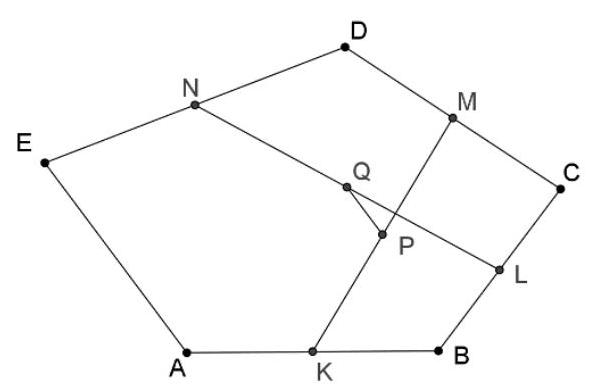
\includegraphics[max width=\textwidth, center]{2024_11_21_fdb726a5bedd0fe80030g-1}\\
której liczby \(\sqrt[3]{3 n}, \sqrt[5]{5 n}\) i \(\sqrt[7]{7 n}\) są naturalne.
  \item Na plażę poszło \(n\) kolegów. Każdy rozłożył na piasku swój ręcznik i poszedł się kąpać. Po godzinie wszyscy wyszli z wody i każdy położył się na losowo wybrany ręcznik. Oznaczmy przez \(p_{k}\) prawdopodobieństwo, że dokładnie \(k\) chłopców trafiło na swój ręcznik. Udowodnij, że
\end{enumerate}

\[
p_{1} \cdot p_{2} \cdot \ldots \cdot p_{n}<0,1
\]


\end{document}